\documentclass[tikz,convert={density=150,size=600,outext=.png}]{standalone}
\usetikzlibrary{shapes, calc, arrows, fit, positioning, decorations, patterns, decorations.pathreplacing, chains, snakes}

\begin{document}
  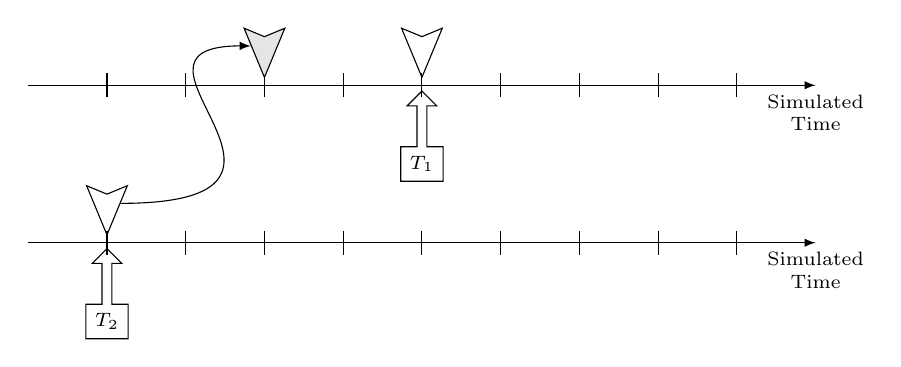
\begin{tikzpicture}[>=latex, font=\scriptsize]
    \draw[->] (0,0) -- (10,0) node[pos=1, below, align=center] (sim-time1) {Simulated\\Time};
    \foreach \x in { 1, 2, 3, 4, 5, 6, 7, 8, 9} {
        \draw (\x,-0.15) -- (\x,0.15) node (tick\x) {};
    };
    \node[draw, arrow box, arrow box arrows={north:.7cm}] at (5, -1) {$T_1$};
    \node[shape=dart, draw, shape border rotate=270 ] at (5, 0.5) {};

    \node[fill=black!10, shape=dart, draw, shape border rotate=270 ] at (3, 0.5) (ev2) {};

    \draw[->] (0,-2) -- (10,-2) node[pos=1, below, align=center] (sim-time2) {Simulated\\Time};
    \foreach \x in { 1, 2, 3, 4, 5, 6, 7, 8, 9} {
        \draw (\x,-2.15) -- (\x,-1.85) node (tick\x) {};
    };

    \node[draw, arrow box, arrow box arrows={north:.7cm}] at (1, -3) {$T_2$};
    \node[shape=dart, draw, shape border rotate=270 ] at (1, -1.5) (ev1) {};

    \draw[->] (ev1.east) .. controls +(3,0) and +(-2,0) .. (ev2.west);
  \end{tikzpicture}
\end{document}
